\section{R : ADTs - Stacks}
\label{chap:adts_stacks}

%%%%%%%%%%%%%%%%%%%%%%%%%%%%%%%%%%%%%%%%%%%%%%%%%%%%%%%%%%%%%%

\begin{frame}[fragile]
\frametitle{ADTs}
\begin{columns}[T]

\begin{column}{0.45\textwidth}
At the highest level of abstraction, ADTs that we can represent
using both dynamic structures (pointers) and also fixed structures (arrays) include:
\begin{itemize}[<+->]
\item Collections (Lists)
\item Stacks
\item Queues
\item Sets
\item Graphs
\item Trees
\end{itemize}
\end{column}

\begin{column}{0.45\textwidth}
\pause
Binary Trees:
\begin{center}
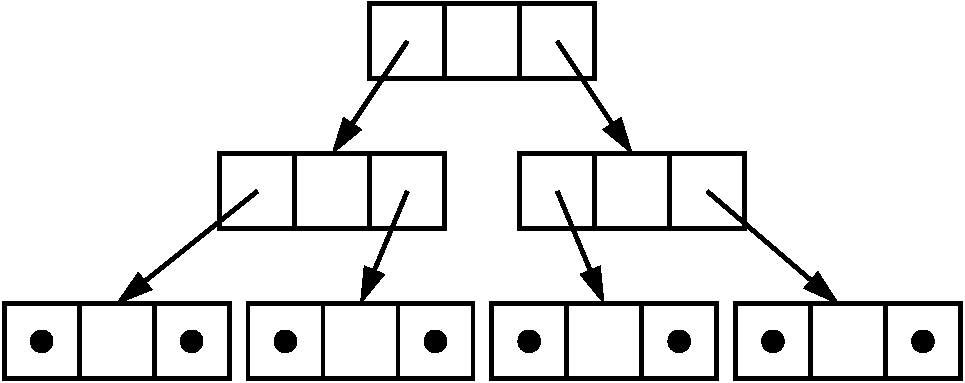
\includegraphics[scale=0.25]{../Images/tree.pdf}
\end{center}
\pause
Unidirectional Graph:
\begin{center}
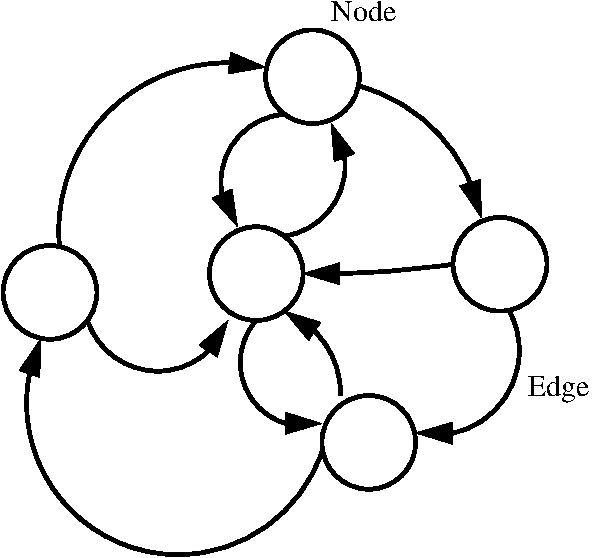
\includegraphics[scale=0.25]{../Images/graph.pdf}
\end{center}
\end{column}

\end{columns}
\end{frame}

%%%%%%%%%%%%%%%%%%%%%%%%%%%%%%%%%%%%%%%%%%%%%%%%%%%%%%%%%%%%%%

\begin{frame}[fragile]
\frametitle{Stacks}
\begin{columns}[T]

\begin{column}{0.45\textwidth}
\begin{center}
The push-down stack:

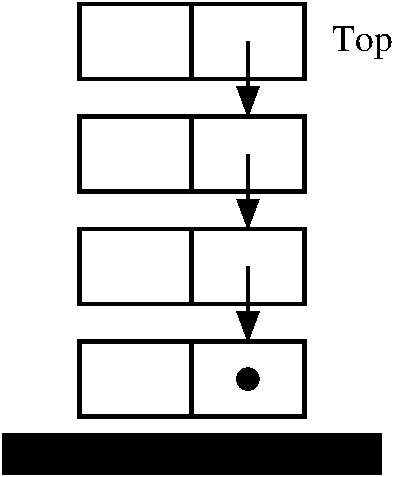
\includegraphics[scale=0.40]{../Images/stack.pdf}
\end{center}
\end{column}

\pause
\begin{column}{0.45\textwidth}
LIFO (Last in, First out):
\begin{center}
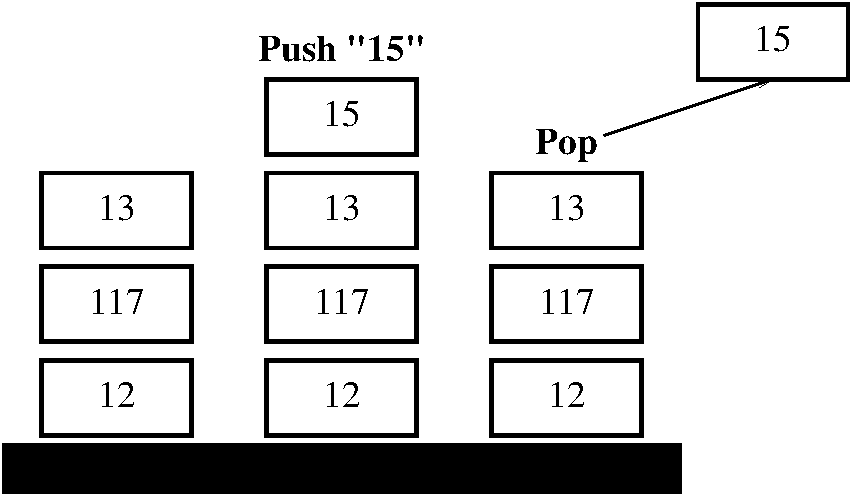
\includegraphics[scale=0.25]{../Images/pdstack.pdf}
\end{center}
\begin{itemize}[<+->]
\item Operations include \verb^push^ and \verb^pop^.
\item In the C run-time system, function calls are implemented using stacks.
\item Most recursive algorithms can be re-written using stacks instead.
\item But, once again, we are faced with the question~: How best to implement such a data type~?
\end{itemize}
\end{column}

\end{columns}
\end{frame}

%%%%%%%%%%%%%%%%%%%%%%%%%%%%%%%%%%%%%%%%%%%%%%%%%%%%%%%%%%%%%%

\begin{frame}[fragile]
\frametitle{ADT:Stacks Arrays (Realloc) I}
\begin{columns}[T]

\begin{column}{0.45\textwidth}
\verb^stack.h:^
\lstinputlisting[style=basicc,linerange={1-30}]{../../ADTs/Stack/stack.h}
\end{column}

\pause
\begin{column}{0.45\textwidth}
\verb^Realloc/specific.h:^
\lstinputlisting[style=basicc]{../../ADTs/Stack/Realloc/specific.h}
\end{column}

\end{columns}
\end{frame}

%%%%%%%%%%%%%%%%%%%%%%%%%%%%%%%%%%%%%%%%%%%%%%%%%%%%%%%%%%%%%%

\begin{frame}[fragile]
\frametitle{ADT:Stacks Arrays (Realloc) II}
\begin{columns}[T]

\begin{column}{0.50\textwidth}
\verb^Realloc/realloc.c^
\lstinputlisting[style=basicc,linerange={1-29}]{../../ADTs/Stack/Realloc/realloc.c}
\end{column}

\pause
\begin{column}{0.40\textwidth}
\lstinputlisting[style=basicc,linerange={31-49}]{../../ADTs/Stack/Realloc/realloc.c}
\end{column}

\end{columns}
\end{frame}

%%%%%%%%%%%%%%%%%%%%%%%%%%%%%%%%%%%%%%%%%%%%%%%%%%%%%%%%%%%%%%

\begin{frame}[fragile]
\frametitle{ADT:Stacks Arrays (Realloc) III}
\begin{columns}[T]

\begin{column}{0.45\textwidth}
\verb^Realloc/realloc.c^
\lstinputlisting[style=basicc,linerange={51-74}]{../../ADTs/Stack/Realloc/realloc.c}
\end{column}

\pause
\begin{column}{0.45\textwidth}
\begin{itemize}[<+->]
\item We need a thorough testing program \verb^teststack.c^
\item See also \verb^revstr.c^ :  a version of the string reverse code (for which we already seen an iterative (in-place) and a recursive solution).
\end{itemize}
\end{column}

\end{columns}
\end{frame}

%%%%%%%%%%%%%%%%%%%%%%%%%%%%%%%%%%%%%%%%%%%%%%%%%%%%%%%%%%%%%%

\begin{frame}[fragile]
\frametitle{ADT:Stacks Linked I}
\begin{columns}[T]

\begin{column}{0.45\textwidth}
\verb^Linked/specific.h^
\lstinputlisting[style=basicc]{../../ADTs/Stack/Linked/specific.h}
\end{column}

\pause
\begin{column}{0.45\textwidth}
\verb^Linked/linked.c^
\lstinputlisting[style=basicc,linerange={1-21}]{../../ADTs/Stack/Linked/linked.c}
\end{column}

\end{columns}
\end{frame}

%%%%%%%%%%%%%%%%%%%%%%%%%%%%%%%%%%%%%%%%%%%%%%%%%%%%%%%%%%%%%%

\begin{frame}[fragile]
\frametitle{ADT:Stacks Linked II}
\begin{columns}[T]

\begin{column}{0.45\textwidth}
\lstinputlisting[style=basicc,linerange={23-44}]{../../ADTs/Stack/Linked/linked.c}
\end{column}

\pause
\begin{column}{0.45\textwidth}
\lstinputlisting[style=basicc,linerange={46-75}]{../../ADTs/Stack/Linked/linked.c}
\end{column}

\end{columns}
\end{frame}
